\documentclass[sigconf,review]{acmart}
\acmConference[MSR 2022]{MSR '22: Proceedings of the 19th International Conference on Mining Software Repositories}{May 23–24, 2022}{Pittsburgh, PA, USA}

% ------------- Packages Used --------------------------------------------------
% They help us to produce a better looking document ;-)
% ------------------------------------------------------------------------------
%\usepackage[tight,footnotesize]{subfigure}

\usepackage{bm}
\usepackage{tabularx}
\usepackage{graphicx}
\usepackage{framed}
\usepackage{colortbl}
\usepackage{balance}
\usepackage{multirow}
\usepackage{booktabs}
\usepackage{varwidth}
\usepackage{collectbox}
\usepackage{comment}
\usepackage{url}
\usepackage{txfonts}
\usepackage{cite}
\usepackage{lscape}
\usepackage{longtable}
\usepackage{caption}
\usepackage{adjustbox}
\usepackage{afterpage}
\usepackage{lipsum}
\usepackage{graphics}
\usepackage{xcolor}

\usepackage{tcolorbox}
\tcbuselibrary{raster,skins}
\definecolor{light-gray}{gray}{0.85}

\usepackage{float}
\usepackage{listings}
\lstset{frame=tb,
  language=Java,
  aboveskip=2mm,
  belowskip=2mm,
  showstringspaces=false,
  columns=flexible,
  basicstyle={\small\ttfamily},
  numbers=none,
  numberstyle=\tiny\color{red},
  keywordstyle=\color{blue},
  commentstyle=\color{red},
  stringstyle=\color{red},
  breaklines=true,
  breakatwhitespace=true,
  tabsize=1
}

%   ACM Style
%\usepackage{lcsect}
% ------------------------------------------------------------------------------

\citestyle{acmauthoryear}
\setcitestyle{numbers,sort&compress}









% ---------- Special commands for annotating the paper's text ------------------
\let\mymarginpar\marginparm
\marginparwidth=1cm
\marginparsep=5pt
\def\fig#1{Figure~\ref{#1}}
\def\tab#1{Table~\ref{#1}}
\def\eqn#1{Equation~\ref{#1}}
\def\sec#1{Section~\ref{#1}}

\usepackage{xspace}
\def\et{et\ al.\xspace}
\def\ie{i.e.\xspace}
\def\eg{e.g.\xspace}
\def\wrt{w.\,r.\,t.\xspace}
\def\aka{a.k.a.\xspace}



\newcommand{\masa}[1]{\textcolor{blue}{{\it [Masa says: #1]}}}



% ------------------------- SYMBOLS OF SELF NAMES OFTEN USED -------------------


% \usepackage[colorlinks,bookmarksopen,bookmarksnumbered,citecolor=red,urlcolor=red]{hyperref}
%\smartqed  % flush right qed marks, e.g. at end of proof
%\smartqed  % flush right qed marks, e.g. at end of proof
%

\usepackage[tight,footnotesize]{subfigure}
\usepackage{cite}
\usepackage{graphicx}
% \usepackage[numbers,sort&compress]{natbib}
% \usepackage{natbib}

\usepackage{comment}


\begin{document}


\title{test}

\author{Hiroki Kuramoto}
\email{kuramoto@posl.ait.kyushu-u.ac.jp}
\author{Hoge hoge}
\email{hoge@posl.ait.kyushu-u.ac.jp}
\author{Hoge hoge}
\email{hoge@posl.ait.kyushu-u.ac.jp}
\author{Hoge hoge}
\email{hoge@posl.ait.kyushu-u.ac.jp}
\additionalaffiliation{Kyushu University}

\begin{abstract}
    test
\end{abstract}
\keywords{GitHub, Video, Image}


\maketitle

\section{Introduction}
\label{sec:intro}
The question ``What makes a good issue report?'' has been studied for decades and is still the ultimate research question for many studies aiming to improve the quality of issue reports~\citep{DBLP:conf/icse/HerzigJZ13}\citep{zimmermann2010TSE}\citep{DBLP:conf/eclipse/BettenburgJSWPZ07}. Issue reports (a.k.a. bug reports) often lack the information necessary for developers to reproduce bugs~\citep{DBLP:conf/msr/JoorabchiMM14}\citep{DearGitHub}. 
For example, Zimmermann~\et~\citep{zimmermann2010TSE} report that stack traces and steps for reproducing a bug are considered to be helpful by developers. But, it is difficult for users to provide this information, and it is often missing or incorrect. 
This mismatch between what developers need and what reporters can provide can often delay the fixing of bugs~\citep{DBLP:conf/msr/JoorabchiMM14}. In addition, many studies have reported that the quality of issue reports impacts both the issue resolution time~\citep{DBLP:conf/cscw/BreuPSZ10}\citep{DBLP:conf/icse/GuoZNM10} and the issue resolution rate~\citep{DBLP:conf/compsac/ZouXZCL15}\citep{DBLP:conf/icse/ZimmermannNGM12}. 

To facilitate developers' bug-reproduction work, GitHub launched a new feature that allows users to share videos (e.g., mp4 files) in May 2021~\citep{github-video-blog}. Using such videos, reports can be made to developers about the details of bugs by recording the symptoms, reproduction steps, and other important aspects of a comprehensive bug report. These visual images can help developers understand the nature of the bug, and what users were doing when the bug occurred. While such visual issue reports have the potential to improve the bug-fixing process, no studies have empirically examined this impact. 

In this paper, we conduct a preliminary study to identify the characteristics of visual issue reports by comparing them with non-visual issue reports.  In addition, we provide the dataset used in this study on a public repository\footnote{\url{https://doi.org/10.5281/zenodo.6071588}}, to promote future studies using visual issue reports. This dataset consists of videos and images in publicly available repositories on GitHub. Specifically, we collected 1,230 videos and 18,760 images from 226,286 issue reports on 4,173 publicly available repositories.


%Our initial analysis reveals that (i) visual issue reports still require reporters to write similar amounts of texts to describe bugs; (ii) visual issue reports are 3-times likely to receive more comments than reports without images or videos; and (iii) resolution time of visual issue reports is longer than that of other issue reports. 
Our initial analysis reveals that 
(i) issue reports with images are described in fewer words than non-visual issues; 
(ii) visual issue reports do not lead to active discussions in the number of words and the first response time; and 
(iii) resolution times of visual issue reports are not significantly changed compared to other issue reports. 
%The main contribution of this paper is opening a new research perspective to study visual issue reports and preparing a new dataset for this research. 
\section{Study Design}
\label{sec:design}

% In this section, we describe the data collection process and 
% the overview of the collected dataset. 
This section describes our study design, including research questions, data collection, metrics computation, and data description.

\subsection{Research Questions}
\label{sec:rqs}

To identify the characteristics of the visual issue reports, we addressed the following three research questions, focusing on Report (RQ1), Discussion (RQ2), and Fix (RQ3). 
\begin{itemize}
	\item[RQ1:] \textbf{\RQone{}}\\
	Developers often suffer from reproducing bugs with the reported information~\citep{DBLP:conf/sigsoft/ChaparroLZMPMBN17}\citep{DBLP:conf/icsm/0001KC20}\citep{zimmermann2010TSE}. 
	On the other hands, as reporters are not always developers, it is not easy to tell what they did and what they encount~\citep{DBLP:conf/sigsoft/ChaparroBLMMPPN19}. Thus, GitHub developed a function that can easily provide information with videos and officially announced the function release on May, 2021~\citep{github-video-blog}. Potter and Faulconer~\citep{POTTER1975} showed that visual images are a more effective approach to describe what people want to communicate and let other people understand it, compared with texts. We hypothesize that videos can reduce the effort for reporting bugs. In this RQ, we measured the number of words in the description of issues as a proxy measure for the effort. 
	\item[RQ2:] \textbf{\RQtwo{}}\\
	We suppose visual issue reports provide 
	more information than the other issue reports. 
	Consequently, developers could discuss the details and 
	result in active discussions. 
	In this RQ, we clarify whether this assumption is true. 
	We measured the activity in terms of 
	the first response time, and
	the number of comments.
	%, and the number of words. 
	\item[RQ3:] \textbf{\RQthree{}}\\
	% We suppose that developers use visualization 
	% in particular issues. 
	% For example, developers may use visualization 
	% to share the way to reproduce bugs. 
	% In this RQ, we clarify the differences 
	% between the issues with and without 
	% visualization. 
	Zimmermann~\et~\citep{zimmermann2010TSE} reported that issue reports occasionally have missing or incorrect steps to reproduce bugs, which delays the entire bug-fixing process~\citep{github-video-blog}. Also, Ohira et al. ~\citep{DBLP:conf/icsm/OhiraHOM12} shows that bug-fixing activities delays when the reporter and developer are different persons because they require communications. Visual issues may mitigate this issue by facilitating their communication. In this RQ, we measure the time from reported to closed to evaluate how quickly visual issue reports are resolved, compared with issues without videos or images. 
\end{itemize}

\subsection{Context Selection}
To select projects as context for our study, we employed \texttt{GHS}\citep{msr2021data}. GHS can find repositories satisfying specific criteria. To filter out unpopular, inactive repositories, or repositories that have no issues, we set up the following criteria.
\begin{itemize}
	\item the number of stars $\geq$ 10
	\item the number of issue reports $\geq$ 1
	\item at least one commit was made in 2021
\end{itemize}
Consequently, the number of the repositories satisfying the criteria was 289,115. From November 2021 to December 2021, we collected 770,656 closed issue reports from 4,173 projects that were randomly selected. While the number of sampled projects seems odds, we collected all the closed issue reports from as many projects as possible in the limited time.  
%As the sampled projects accounts for only less than 2\% of all repositories, we discuss the threat to validity of this process in \sec{sec:limitation}. 


% 
\begin{figure*}[t]
\centering
% 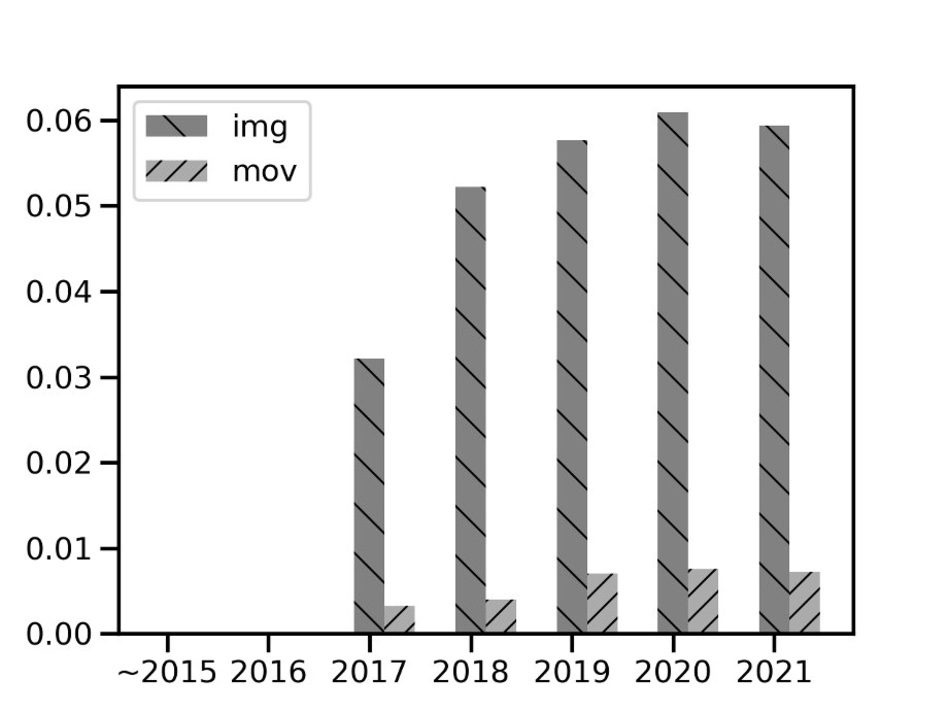
\includegraphics[width=1\linewidth]{./figures/data-category-trend.pdf}
\caption{ 
  An overview of the data collection
  }
\label{fig:data-collection-overview}
\end{figure*}


\subsection{Data Collection}
%\fig{fig:data-collection-overview} shows an overview of the data collection process. 
We first collected closed issue reports with \texttt{PyGitHub}\footnote{\url{https://pygithub.readthedocs.io/en/latest/index.html}} that internally execute GitHub API v3\footnote{\url{https://docs.github.com/en/rest}}. 
Next, we collected videos and images attached to the issue reports. While GitHub users can see videos and images on issue pages, the videos and images are stored in different URLs. As the URLs are written in the text description of issue reports, we parsed them with regular expressions and downloaded them. The regular expressions we used are shown as follows:
\begin{quote}
\addtolength\leftmargini{0in}
{\it https://user-images.githubusercontent.com/[a-zA-Z0-9\textbackslash-/]+\textbackslash.[a-zA-Z0-9]+}
\end{quote}
Each downloaded file was determined to be a image or video by its extension. Specifically, png, PNG, jpg, JPG, and jpeg are treated as images, and  gif, GIF, mp4, MP4, and mov as videos.
Consequently, we downloaded 33,079 images and 3,819 movies
with the collected URLs.\masa{to kuramoto: i wrote these numbers. are the numbers correct?} 


% \begin{table*}[h]
    \begin{center}
    \caption{Examples of the retrieved issues with the values of the attributes}
    \begin{tabular}{c c c c c c c} 
      \toprule
      \textbf{IssueCreatedYear} &
      \textbf{ResolutionTime} &
      \textbf{Images} &
      \textbf{Videos} &
      \textbf{Comments} &
      \textbf{FirstCommentTime} &
      \textbf{DescriptionLength} \\
      \midrule
      2020 & 6.99861111 & 0 & 0 & 1 & 6.99861111 & 4430\\
      2020 & 41.9594329 & 1 & 0 & 3 & 17.7784722 & 85\\
      2020 & 43.8850579 & 0 & 0 & 2 & 0.49828704 & 56\\
      2020 & 44.0935532 & 0 & 0 & 4 & 0.91277778 & 33\\
      2020 & 0.14934028 & 0 & 0 & 8 & 0.08077546 & 244\\
      2020 & 59.5670949 & 2 & 0 & 5 & 0.39472222 & 102\\
      2020 & 74.9322569 & 0 & 0 & 0 & -          & 24\\
      \bottomrule
    \end{tabular}
    \label{tab:example-dataset}
    \end{center}
  \end{table*}

% We extract a part of the retrieved issues in \tab{tab:example-dataset}. 
% Each row corresponds to the values of the attributes of an issue. 
%
\begin{table}[t]
    \begin{center}
    \caption{The attributes we collected from the issues}
    \scalebox{0.85}[0.85]{
    \begin{tabular}{ll} 
        \toprule
        \multicolumn{1}{c}{\textbf{Attributes}} & \multicolumn{1}{c}{\textbf{Description}} \\ 
        \midrule
        $IssueResolvedTime$ & The time until the issue is resolved (day) \\
        $FirstCommentTime$ & The time until the first comment (day) \\
        $\#comments$ & The number of comments \\
        $\#chars$ & \masa{im not sure what is this} \\
        $\#imgs$ & \# of attached images when the issue is created \\
        $\#movs$ & \# of attached movies when the issue is created \\
        $\#words$ &  \masa{im not sure what is this} \\
        $IssueCreatedYear$ & The year when the issue is created \\
        \bottomrule
    \end{tabular}
    }
    \label{tab:issue-attr}
    \end{center}
\end{table}


\begin{table}[t]
    \begin{center}
    \caption{The attributes we collected from the issues}
    \scalebox{0.85}[0.85]{
    \begin{tabular}{ll} 
        \toprule
        \multicolumn{1}{c}{\textbf{Attributes}} & \multicolumn{1}{c}{\textbf{Description}} \\ 
        \midrule
        $IssueResolvedTime$ & The time until the issue is resolved (day) \\
        $FirstCommentTime$ & The time until the first comment (day) \\
        $\#comments$ & The number of comments \\
        $\#chars$ & \masa{im not sure what is this} \\
        $\#imgs$ & \# of attached images when the issue is created \\
        $\#movs$ & \# of attached movies when the issue is created \\
        $\#words$ &  \masa{im not sure what is this} \\
        $IssueCreatedYear$ & The year when the issue is created \\
        \bottomrule
    \end{tabular}
    }
    \label{tab:issue-attr}
    \end{center}
\end{table}

\subsection{Analysis}
We retrieved the attributes from the collected issue reports.
\tab{tab:issue-attr} shows seven attributes extracted from 
the issue reports. 
The attributes can be classified into three dimensions, 
``Report'', ``Discussion'', and ``Fix''. 
The attributes in the dimension ``Report'' are extracted from 
the description of issue reports or attached files 
when the issue was created. 
In particular, in RQ1, we 
%calculate 
utilize the number of words 
in reports (\ie, $DescriptionLength$) for Img, Vid, and None. 
In addition,  $\#imgs$ and $\#vids$ are used to show 
dataset description. 
Note that these attributes are not calculated from either title, not comments (i.e., only descriptions were used). 
Also, when computing $DescriptionLength$, if the description of the issue report 
includes URLs for images/videos, 
we exclude them from the description because these are not words.

The dimension ``Discussion'' has two attributes, $Comments$ and $FirstCommentTime$. $Comments$ is the number of comments were made in the issue report. We utilize this attribute as a proxy measure of discussion effort. $FirstCommentTime$ is the days subtract from when the first comment was made to when issue was reported. We employ this attribute for measuring developers' interest. 

The dimension ``Fix'' has one attribute $IssueResolvedTime$ which shows the time from reported to fixed. 
Note that some negative values of $IssueResolvedTime$ were observed. We investigated it manually and found that these are because of a bug in GitHub.  We excluded those issues that have negative values from our dataset. 
In addition, we excluded issue reports resolved in too short or long periods (e.g., 30 seconds) because they might be issued after being fixed or might not be fixed in reality.
%\kashiwa{check please}
Specifically, we only use the issue reports that meet the condition: $30\ sec \leq IssueResolvedTime \leq 1\ year$.
The number of issue reports that meet this condition is 711,160 (92.23\%).


\kashiwa{Write what do you analyze (e.g., compare them in median)}
To evaluate the difference, we used a non-parametric test \textit{Steel-Dwass test}.
\kashiwa{Write what this test is}
\kashiwa{Write why this test is selected}
because our preliminary study shows that 
the distributions for each category do not 
come from normal distributions.
\kashiwa{Write the reason why correction is not needed (i.e., how to deal with family-wise error rate)}

\section{Future Research Plan}
\label{sec:future}



% \section{Limitation}
\subsection{Threats to Validity}
\label{sec:limitation}

While the number of issue reports that we studied is 770,656,  this number accounts for only less than 2\% of all the repository due to the time limitation. 
We believe that the selection of repositories is not biased because we randomly selected these repositories. 
Still, we cannot generalizerize the findings in this study. 

In addition, since GitHub released the feature to post videos in May 2021, this feature is still new and yet to be common. The number of visual issue reports has increased as \fig{fig:data-cat-trend} shows, and then the results may vary after the feature becomes popular. 

We collected the issue reports with PyGitHub. 
However, in this process, some pull requests were also collected due to the specification of GitHub. 
Hence, our analysis may include such pull requests as issue reports. \kashiwa{RECHECK}
\section{Conclusion}
\label{sec:conclusion}

\masa{conclusion here}

Finally, we present future research directions with our dataset. 


\noindent
\textbf{The impact analysis of movies and images on software development.}
GitHub added the feature~\citep{github-video-blog} to easily 
share movies with GitHub to earn advantages 
in software development such as reproducing bugs easily in issues and 
explaining the background of changes in pull requests. 
However, no studies exist that investigate whether such movies 
impact software development. 
Hence, investigating the impact of movies on software development 
is a future research direction. 
Specifically, we study the reduction of issue resolution time, 
the response rate of developers, and 
the reduction of the number of comments 
in which developers write ``works for me''. 

\noindent
\textbf{Automated bug reproduction with image processing.}
Reproducing bugs is a time-consuming process 
in software development\masa{citation}.
Automating this process would support developers 
to quickly find and fix the cause of bugs. 
Hence, it is an important future research direction 
to automate bug reproduction. 
As the evolution of image processing with deep learning models, 
the accuracy of image processing significantly improves\masa{citation}. 
Hence, we apply such deep learning models to movies 
to implement automated bug reproduction tools. 


\section*{Acknowledgment}
This work has been supported by JSPS KAKENHI Japan
(Grant Numbers: \masa{update}.


\bibliographystyle{ACM-Reference-Format}
\bibliography{reference}



\end{document} 
